\documentclass[14pt,fleqn]{extarticle}
\RequirePackage{prepwell}
\previewoff
\begin{document}

%text
Find the volume of the largest cylinder that
can be inscribed in a sphere of radius $R$. 
%

\newcard

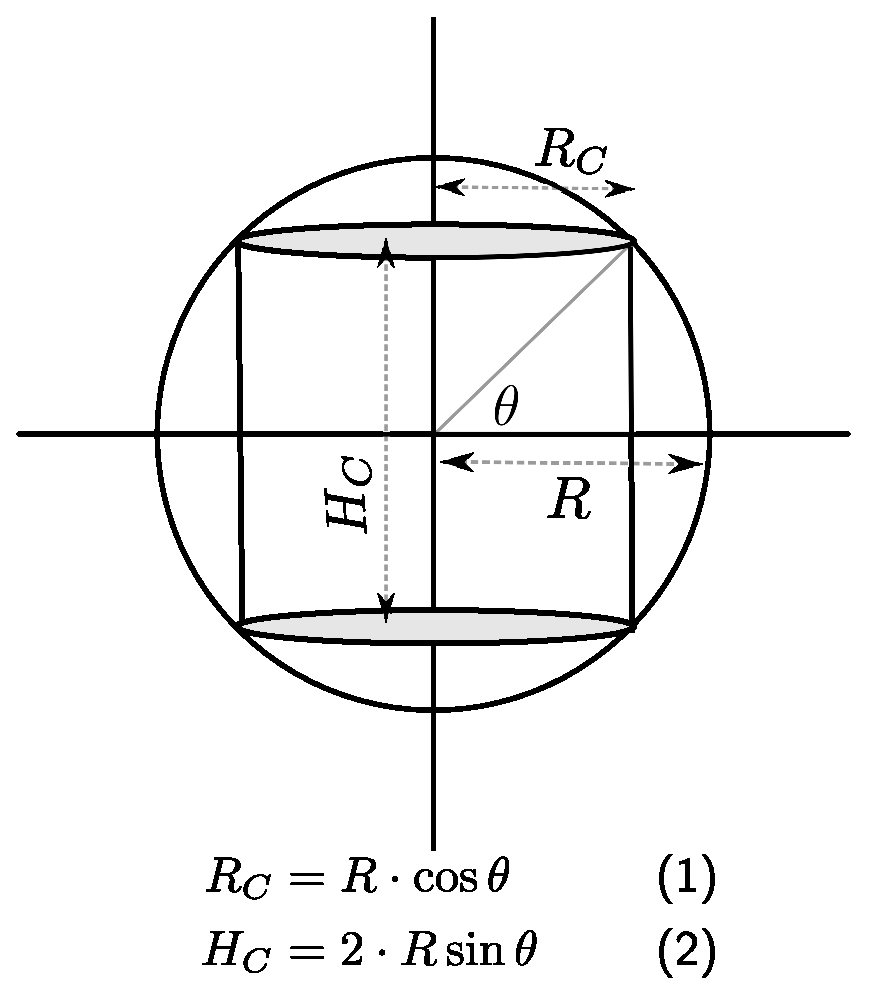
\includegraphics[scale=0.5]{right.eps}

\newcard 

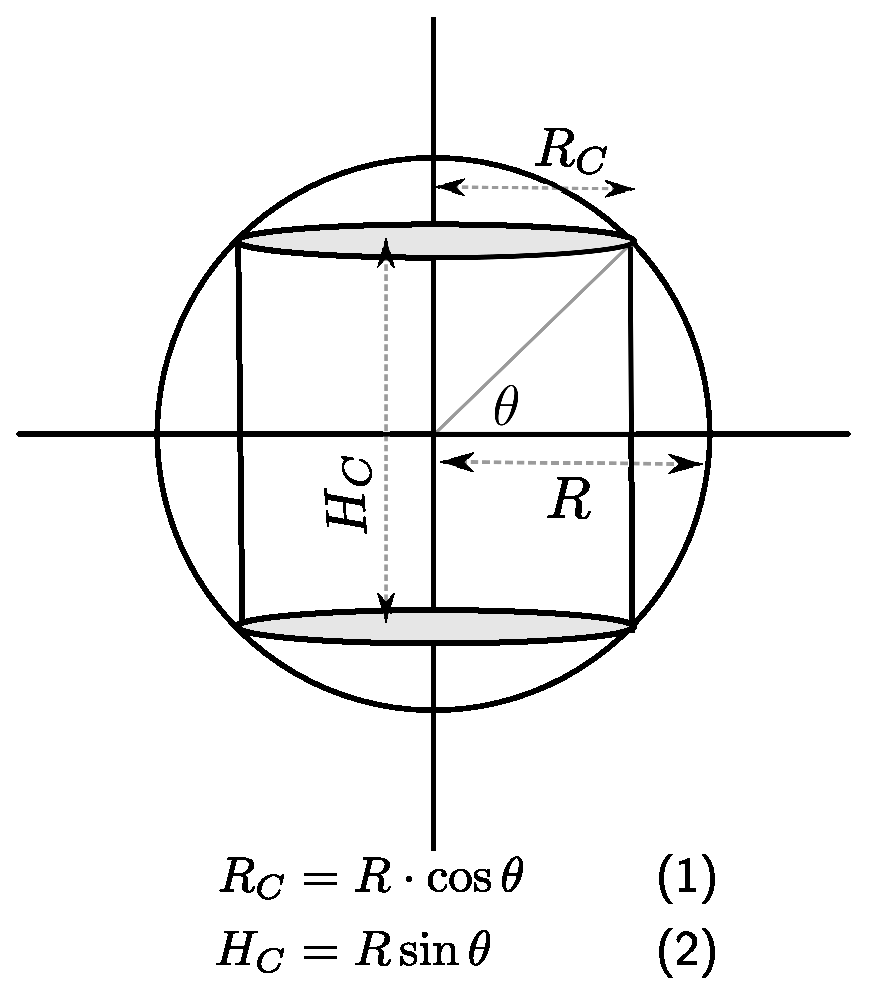
\includegraphics[scale=0.5]{wrong.eps}

\newcard

The cylinder is \underline{inside the sphere}. Moreover, one can see from the diagram that 

\[ \quad \cos\theta = \frac{R_C}{R} \text{ and } \frac{H_C}{2} = R\cdot \sin\theta \]

This means that 
\[ \quad R_C = R\cdot\cos\theta \text{ and } H_C = 2R\cdot\sin\theta \]

The idea is to deal with only one variable $(\theta)$ instead of two -- $R_C\text{ and } H_C$ 

\newcard 

\begin{align}
	V &= 2\pi R^2\cdot \left(\sin\theta - \sin^3\theta \right) \\
	\therefore \frac{dV}{d\theta} &= 0\implies\theta = \sin^{-1}\frac{1}{\sqrt{3}} \,\left(\text{or }\theta = \tan^{-1}\frac{1}{\sqrt{2}} \right)
\end{align}

\newcard 

The volume of the given cyclinder is 

\begin{align}
	V &= \left(\pi\cdot R_C^2 \right)\cdot H_C = \left(\pi\cdot R^2\cos^2\theta \right)\cdot 2R\sin\theta \\
	&= \left(2\pi R^3 \right)\cdot \left(\cos^2\theta\cdot \sin\theta \right) \\	
	&= 2\pi\cdot R^3 \left[\left(1-\sin^2\theta \right)\cdot \sin\theta \right] \\
	&= 2\pi R^3 \left[\sin\theta-\sin^3\theta \right] \\
	\therefore \frac{dV}{d\theta} &= 2\pi R^3\cdot \left[\cos\theta - 3\sin^2\theta\cos\theta \right] \\
	&= 2\pi R^3\cdot\cos\theta\cdot \left(1-3\sin^2\theta \right) \\
	\text{Hence, } \frac{dV}{d\theta} &= 0 \implies \cos\theta = 0\text{ or } \sin\theta = \frac{1}{\sqrt{3}} \\
	\cos\theta &= 0 \implies \theta = \frac\pi{2}\implies \underbrace{R_C = 0}_{\text{No cylinder}}\\
	\therefore \theta &= \sin^{-1}\frac{1}{\sqrt{3}} 
\end{align}

\newcard

Hence, the \underline{maximum volume} $V_m$ is 
\[ \quad \qquad V_m = \frac{4\pi R^3}{3\sqrt{3}} \] 

\newcard 

Hence, the \underline{maximum volume} $V_m$ is 
\[ \quad \qquad V_m = \frac{2\pi R^3}{\sqrt{3}} \] 


\newcard 

We found that at $\theta = \sin^{-1}\frac{1}{\sqrt{3}}$, the cylinder has an 
\underline{extreme} value (a maxima or a minima). But which is it? \newline 

Now, ordinarily, you would calculate $\frac{d^2 V}{d\theta^2}$ also and infer 
the nature of the extrema (maxima or minima) \newline 

But in this case, you know that $\theta=\sin^{-1}\frac{1}{\sqrt{3}}$ is \underline{not a minima}\newline 

Why? Because as $\theta\to\frac\pi{2}, V\to 0$. In fact, the minimum value of $V$ is 0 at $\theta=\frac\pi{2}$. No other minimum value is possible \newline 

Hence, the extreme point we found must be the maxima \newline 

And the maximum volume is 

\begin{align}
	V_m &= \left(\pi R^2\cos^2\theta \right)\cdot \left( 2R\sin\theta \right) \\
	\text{where }\sin\theta &= \frac{1}{\sqrt{3}}\implies\cos\theta = \sqrt\frac{2}{3} \\
	\therefore V_m &= \pi R^2\frac{2}{3}\cdot 2 R\cdot \frac{1}{\sqrt{3}} = \dfrac{4\pi R^3}{3\sqrt{3}} 
\end{align}

\end{document}